\documentclass[a4paper,11pt]{ujreport}
%%【PostScript, JPEG, PNG等の画像の貼り込み】
%% 利用するパッケージを選んでコメントアウトしてください.
\usepackage{graphicx} % for 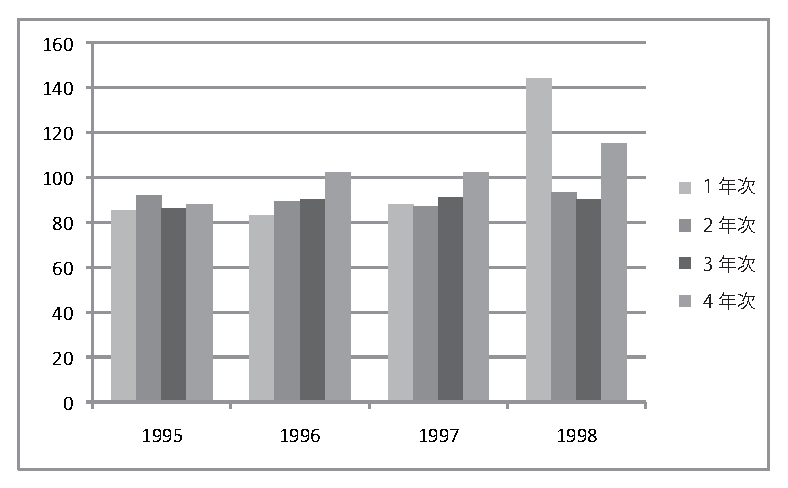
\includegraphics[width=3cm]{sample.eps}
\usepackage{epsfig} % for 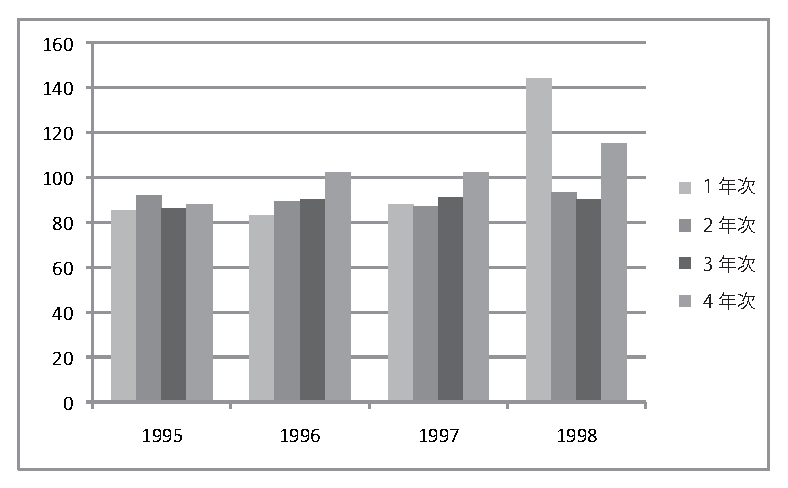
\psfig{file=sample.eps,width=3cm}
%\usepackage{epsf} % for \epsfile{file=sample.eps,scale=0.6}
%\usepackage{epsbox} % for \epsfile{file=sample.eps,scale=0.6}
\usepackage{/Users/takagihayata/workspace/materialize-mongodb/paper/mast/class/mediabb} % for pdf

\usepackage{times} % use Times Font instead of Computer Modern
% \usepackage{listings} % for soursecode
% \usepackage{plistings} % for soursecode
\usepackage{/Users/takagihayata/workspace/materialize-mongodb/paper/mast/class/docmute} % texファイル分割用

\setcounter{tocdepth}{3}
\setcounter{page}{-1}

\setlength{\oddsidemargin}{0.1in}
\setlength{\evensidemargin}{0.1in}
\setlength{\topmargin}{0in}
\setlength{\textwidth}{6in}
%\setlength{\textheight}{10.1in}
\setlength{\parskip}{0em}
\setlength{\topsep}{0em}

%\newcommand{\zu}[1]{{\gt \bf 図\ref{#1}}}

%% タイトル生成用パッケージ(重要)
\usepackage{/Users/takagihayata/workspace/materialize-mongodb/paper/mast/class/mast-jp-sjis}

%% タイトル
%% 【注意】タイトルの最後に\\ を入れるとエラーになります
\title{NoSQL型データベースシステムでの実体化ビュー選択に関する研究}
%% 著者
\author{髙木 颯汰}
%% 指導教員
\advisor{古瀬 一隆 陳 漢雄}

%% 年月 (提出年月)
%% 年月は必要に応じて書き替えてください.
\majorfield{ } \yearandmonth{2019年 1月}


\addtocounter{page}{2} %単体でコンパイルした際の調整用
\addtocounter{chapter}{4} %単体でコンパイルした際の調整用
\begin{document}

\chapter{結果・考察}
\label{chap:Result}
\section{実験Aの結果}
実験結果を図\ref{ExperimentA-find},\ref{ExperimentA-update},\ref{ExperimentA-total}に示す.図\ref{ExperimentA-find},\ref{ExperimentA-update}は各コレクションにおけるクエリの平均処理時間を示している.図\ref{ExperimentA-total}は検索処理と更新処理の累計処理時間を示している.
\begin{figure}[htbp]
	\begin{center}
		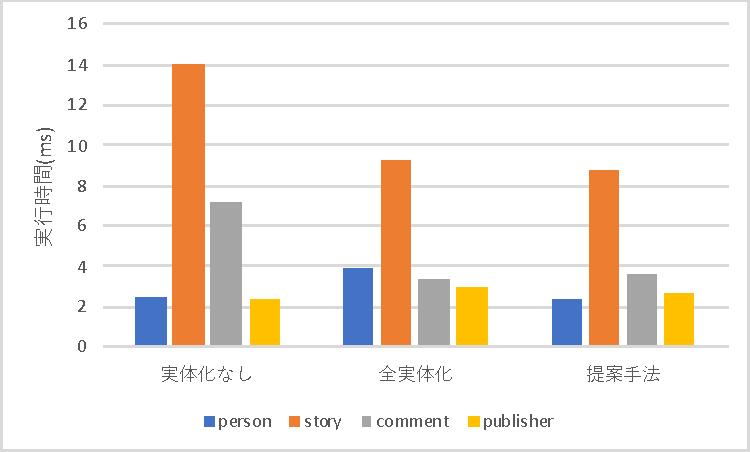
\includegraphics[width=30em]{src/ExperimentA-find.pdf} %[trim=left bottom right top]
	\end{center}
	\caption{実験Aの各コレクションの平均検索時間}
	\label{ExperimentA-find}
\end{figure}
\begin{figure}[htbp]
	\begin{center}
		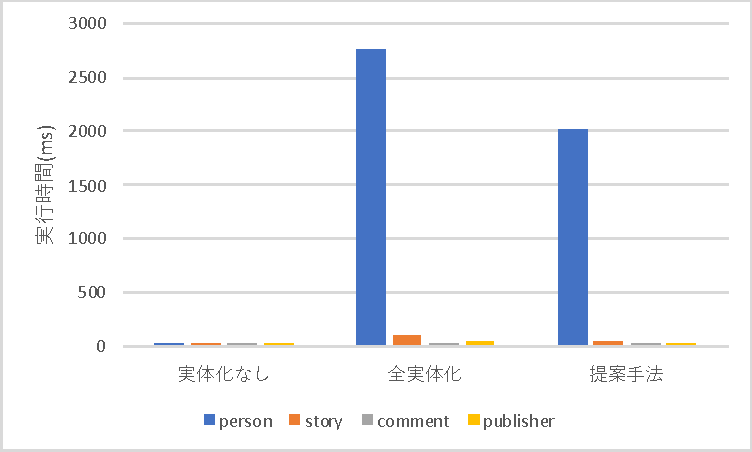
\includegraphics[width=30em]{src/ExperimentA-update.pdf} %[trim=left bottom right top]
	\end{center}
	\caption{実験Aの各コレクションの平均更新時間}
	\label{ExperimentA-update}
\end{figure}
\begin{figure}[htbp]
	\begin{center}
		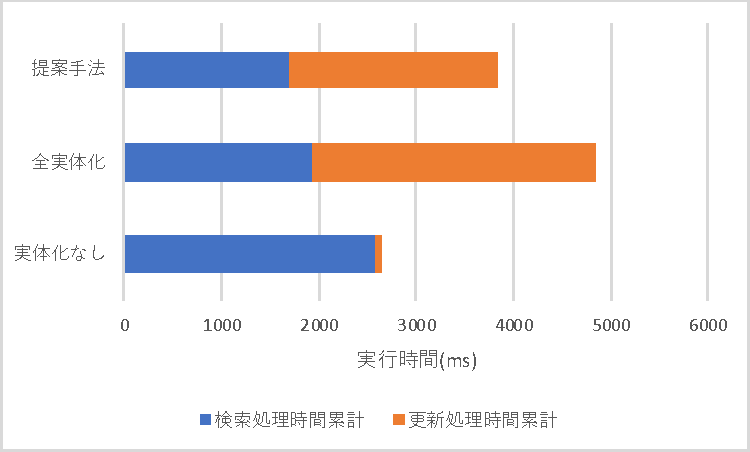
\includegraphics[width=30em]{src/ExperimentA-total.pdf} %[trim=left bottom right top]
	\end{center}
	\caption{実験Aの累計処理時間}
	\label{ExperimentA-total}
\end{figure}

\section{実験Bの結果}
実験結果を図\ref{ExperimentB-find},\ref{ExperimentB-update},\ref{ExperimentB-total}に示す.図\ref{ExperimentB-find},\ref{ExperimentB-update}は各コレクションにおけるクエリの平均処理時間を示している.図\ref{ExperimentB-total}は検索処理と更新処理の累計処理時間を示している.検索処理速度に関しては全実体化と提案手法が実体化なしのデータモデルより速い結果となった.一方,更新処理速度は実体化なしのデータモデルが最速であり,personコレクションに関しては全実体化と提案手法でのデータモデルが実体化なしと比べて100倍程遅い結果となった.
\begin{figure}[htbp]
	\begin{center}
		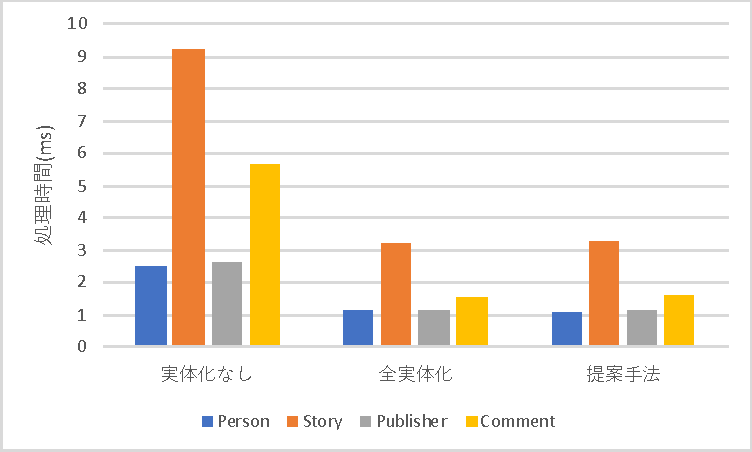
\includegraphics[width=30em]{src/ExperimentB-find.pdf} %[trim=left bottom right top]
	\end{center}
	\caption{実験Bの各コレクションの平均検索時間}
	\label{ExperimentB-find}
\end{figure}
\begin{figure}[htbp]
	\begin{center}
		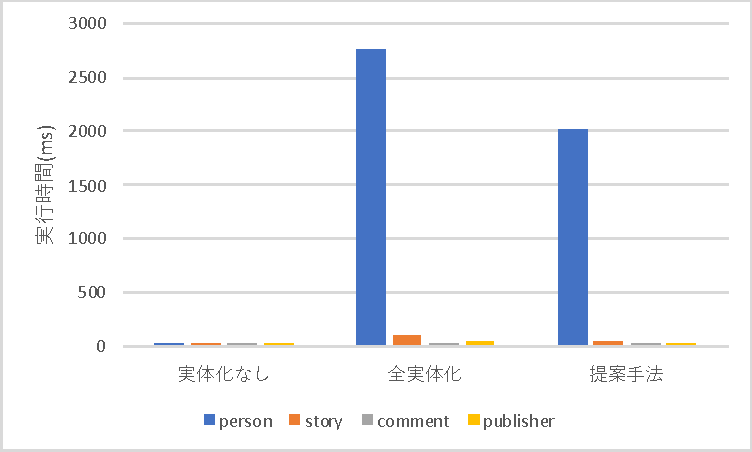
\includegraphics[width=30em]{src/ExperimentB-update.pdf} %[trim=left bottom right top]
	\end{center}
	\caption{実験Bの各コレクションの平均更新時間}
	\label{ExperimentB-update}
\end{figure}
\begin{figure}[htbp]
	\begin{center}
		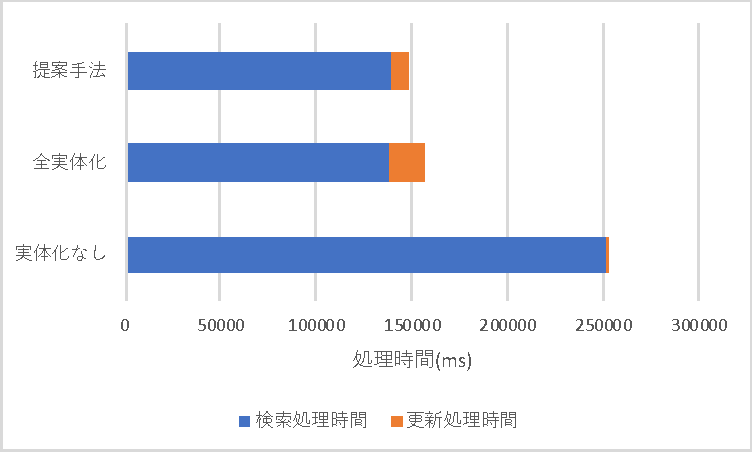
\includegraphics[width=30em]{src/ExperimentB-total.pdf} %[trim=left bottom right top]
	\end{center}
	\caption{実験Bの累計処理時間}
	\label{ExperimentB-total}
\end{figure}

\section{実験Cの結果}
実験結果を図\ref{ExperimentC-find},\ref{ExperimentC-update},\ref{ExperimentC-total}に示す.実験Bと同じく,検索処理で全実体化と提案手法が実体化なしと比べて1.5倍から2倍早く,更新処理で全実体化と提案手法が実体化なしと比べて100倍程度遅い結果となった.
\begin{figure}[htbp]
	\begin{center}
		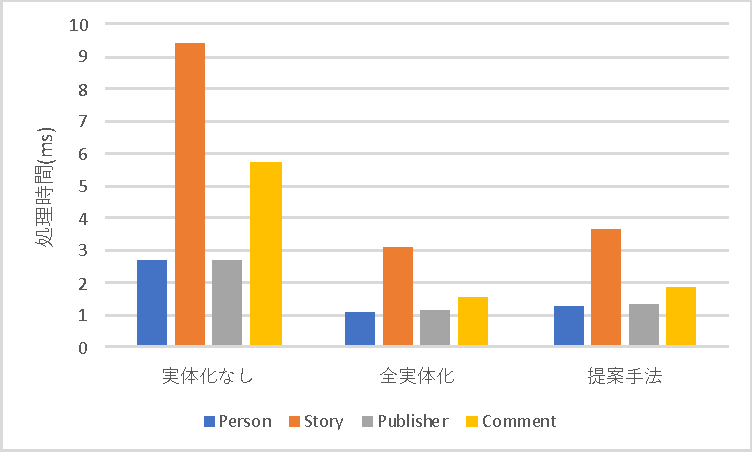
\includegraphics[width=30em]{src/ExperimentC-find.pdf} %[trim=left bottom right top]
	\end{center}
	\caption{実験Cの各コレクションの平均検索時間}
	\label{ExperimentC-find}
\end{figure}
\begin{figure}[htbp]
	\begin{center}
		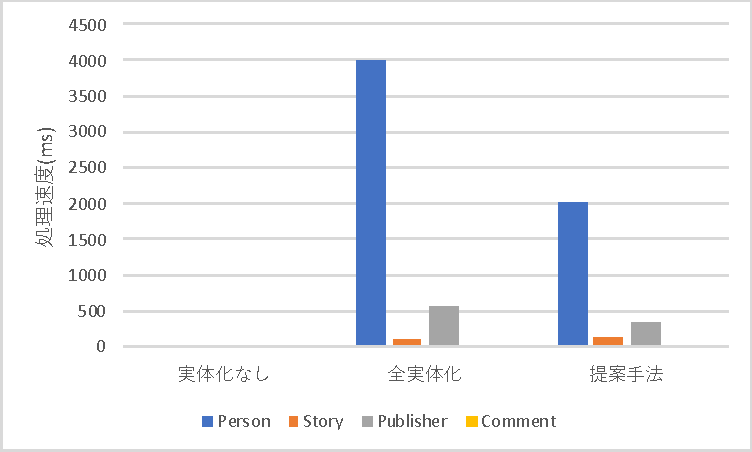
\includegraphics[width=30em]{src/ExperimentC-update.pdf} %[trim=left bottom right top]
	\end{center}
	\caption{実験Cの各コレクションの平均更新時間}
	\label{ExperimentC-update}
\end{figure}
\begin{figure}[htbp]
	\begin{center}
		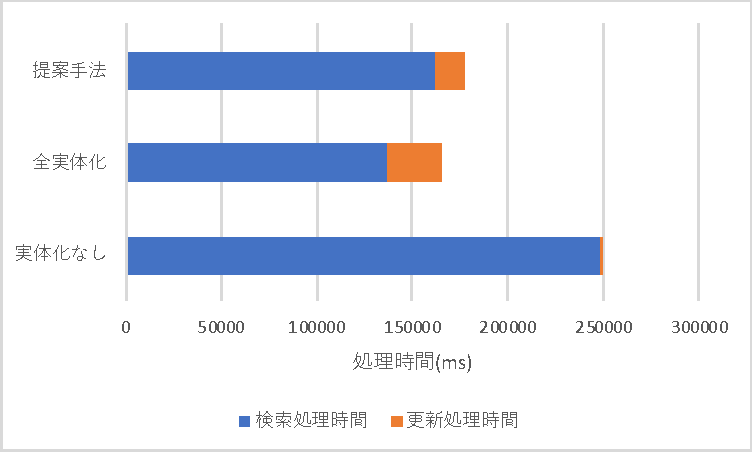
\includegraphics[width=30em]{src/ExperimentC-total.pdf} %[trim=left bottom right top]
	\end{center}
	\caption{実験Cの累計処理時間}
	\label{ExperimentC-total}
\end{figure}

\section{実験Dの結果}
実験結果を図\ref{ExperimentD-find},\ref{ExperimentD-update},\ref{ExperimentD-total}に示す.概ね実験B,Cと同じで,実体化なしと比べて全実体化と提案手法が1.5倍~2倍検索処理で速く,更新処理で遅い結果となった.更新時間では全実体化と比べて提案手法が2倍程度速い結果となった.
\begin{figure}[htbp]
	\begin{center}
		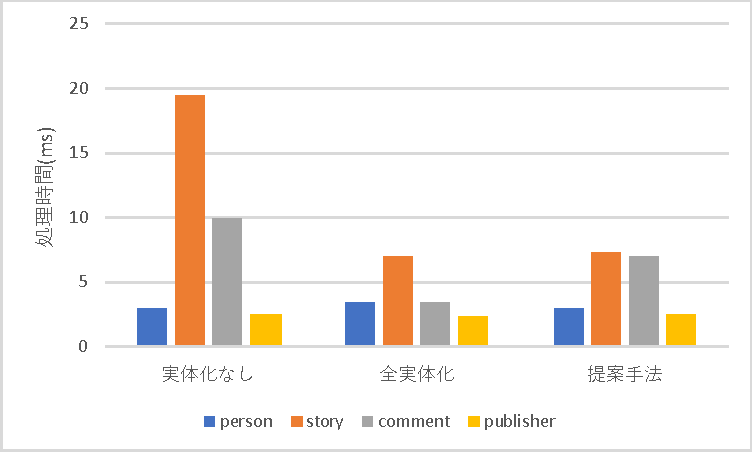
\includegraphics[width=30em]{src/ExperimentD-find.pdf} %[trim=left bottom right top]
	\end{center}
	\caption{実験Dの各コレクションの平均検索時間}
	\label{ExperimentD-find}
\end{figure}
\begin{figure}[htbp]
	\begin{center}
		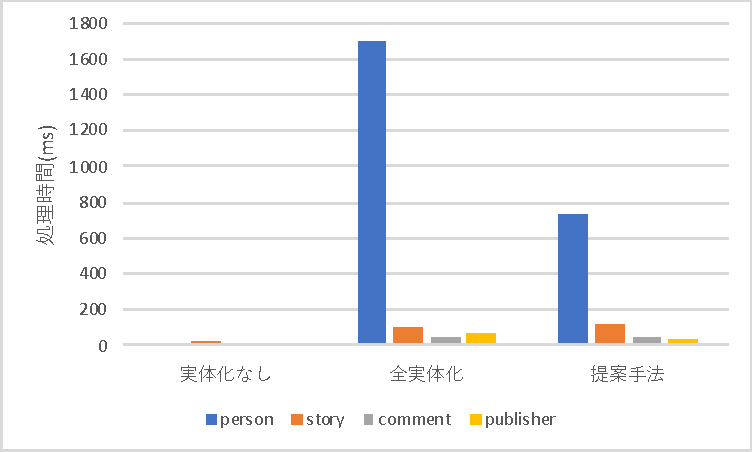
\includegraphics[width=30em]{src/ExperimentD-update.pdf} %[trim=left bottom right top]
	\end{center}
	\caption{実験Dの各コレクションの平均更新時間}
	\label{ExperimentD-update}
\end{figure}
\begin{figure}[htbp]
	\begin{center}
		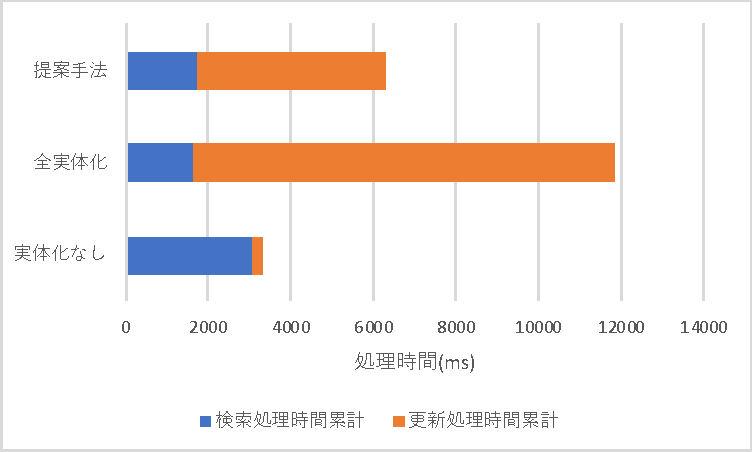
\includegraphics[width=30em]{src/ExperimentD-total.pdf} %[trim=left bottom right top]
	\end{center}
	\caption{実験Dの累計処理時間}
	\label{ExperimentD-total}
\end{figure}

\section{実験Eの結果}
実験結果を図\ref{ExperimentE-find},\ref{ExperimentE-update},\ref{ExperimentE-total}に示す.実験Dと同様に実体化なしと比べて全実体化と提案手法が検索処理で速く,更新処理で遅い結果であり,提案手法は全実体化と比べて2倍程度更新速度が速い結果となった.それに付随して,累計処理時間も提案手法が全実体化と比べて2倍程度速い結果となっている.
\begin{figure}[htbp]
	\begin{center}
		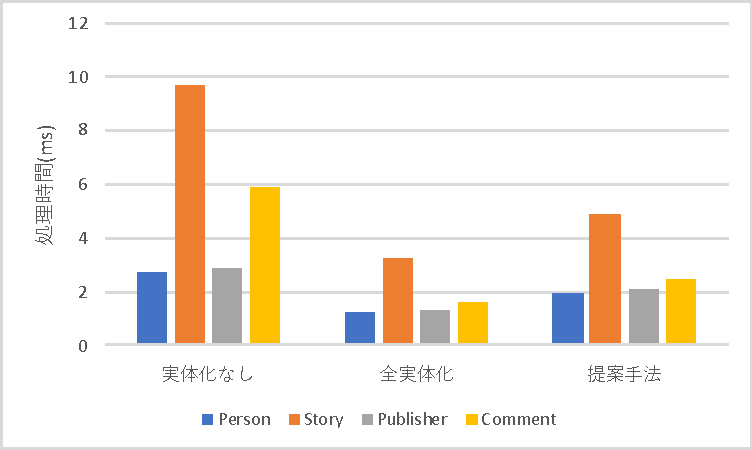
\includegraphics[width=30em]{src/ExperimentE-find.pdf} %[trim=left bottom right top]
	\end{center}
	\caption{実験Eの各コレクションの平均検索時間}
	\label{ExperimentE-find}
\end{figure}
\begin{figure}[htbp]
	\begin{center}
		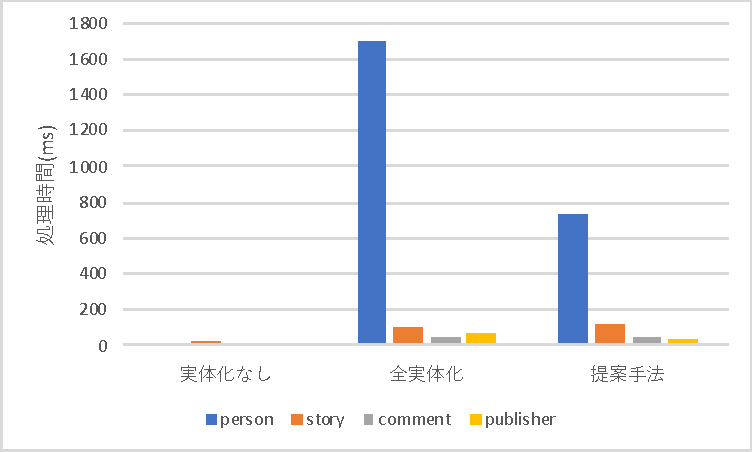
\includegraphics[width=30em]{src/ExperimentE-update.pdf} %[trim=left bottom right top]
	\end{center}
	\caption{実験Eの各コレクションの平均更新時間}
	\label{ExperimentE-update}
\end{figure}
\begin{figure}[htbp]
	\begin{center}
		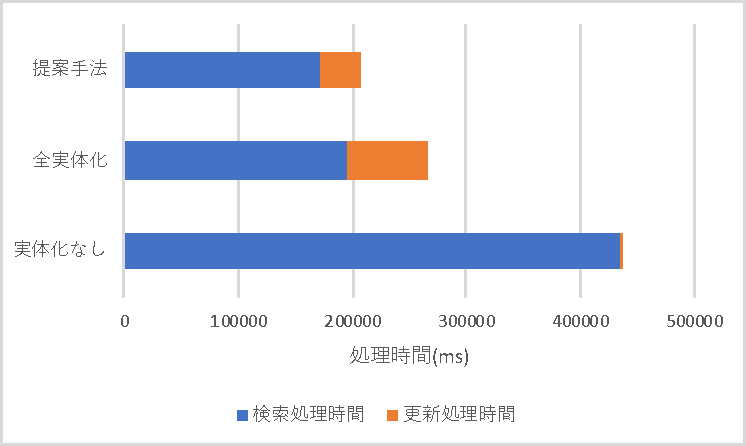
\includegraphics[width=30em]{src/ExperimentE-total.pdf} %[trim=left bottom right top]
	\end{center}
	\caption{実験Eの累計処理時間}
	\label{ExperimentE-total}
\end{figure}

\section{実験の考察}
\label{sec:Consideration}
全実体化と提案手法は実体化なしと比べて累計検索処理時間が約半減した.通常であれば元のクエリに加えて結合先のクエリをMongoDB発行しアプリケーション層でドキュメントを結合するが,Materialized Viewを用いた場合には追加のクエリ発行と結合処理を省くことができる.その為,結合処理が発生するstory,commentコレクションの検索時間が高速化した.

実験を通して実体化した場合には更新時間が増大した.これはオリジナルのドキュメントに加えて,そのドキュメント自体のMaterialized Viewと,ドキュメントが埋め込まれているMaterialized Viewを更新する必要があり.MongoDB側に発行するクエリが増えるからである.今回の実験ではstoryコレクションに最大100のpersonドキュメントが埋め込まれており,personドキュメントを更新する際には実体化したpersonドキュメントと,そのドキュメントが埋め込まれているstoryドキュメントを更新する必要がある.実際に,実験Eではユーザーからのpersonコレクションへの9つのクエリに対してミドルウェアで521のクエリを発行していた.

実験D,Eでは全実体化と比べて提案手法の更新処理時間が1/2になっている.これは実験B,Cと比べて更新のクエリが増えて実体化条件で用いるデータが増え,実体化選択の精度が上がったと考えられる.


\end{document}
